\documentclass[11pt,a4paper]{article}
\usepackage[utf8]{inputenc}
\usepackage{geometry}
\usepackage{graphicx}
\usepackage{titlesec}
\usepackage{parskip}
\usepackage{listings}
\usepackage{xcolor}
\usepackage{float}
\usepackage{hyperref}
\usepackage{enumitem}
\usepackage{tikz}
\usetikzlibrary{shapes.geometric, arrows.meta, positioning, fit, backgrounds, calc}

\geometry{margin=2.5cm}

% Configuração de código
\lstset{
    basicstyle=\small\ttfamily,
    breaklines=true,
    frame=single,
    numbers=left,
    numberstyle=\tiny,
    commentstyle=\color{gray},
    keywordstyle=\color{blue},
    stringstyle=\color{red}
}

% Formatação de títulos
\titleformat{\section}{\Large\bfseries}{\thesection}{1em}{}
\titleformat{\subsection}{\large\bfseries}{\thesubsection}{1em}{}

\begin{document}

% PÁGINA DE CAPA
\begin{titlepage}
    \centering
    
    % Logo e identificação institucional
    \includegraphics[width=0.3\textwidth]{logoUminho.png}\\[0.5cm]
    
    {\large \textbf{Universidade do Minho}}\\[0.3cm]
    {\large Escola de Engenharia}\\[0.2cm]
    {\large Departamento de Informática}\\[3cm]
    
    % Título principal
    {\Huge \textbf{Sistema de Séries Temporais\\[0.3cm]Distribuído}}\\[1cm]
    
    % Contexto académico
    {\Large Sistemas Distribuídos}\\[0.3cm]
    {\large Trabalho Prático}\\[0.3cm]
    {\large Ano Letivo 2025/2026}\\[3cm]
    
    % Identificação do grupo (alinhado à direita)
    \begin{flushright}
        \textbf{Grupo 15}\\[0.5cm]
        Rui Morais - A76650\\
        Carlos Silva - A106792\\
        Francisco Soares - A106882\\
        Nuno Soares - A107366\\
    \end{flushright}
    
    \vfill
    
    % Data
    {\large Janeiro de 2026}
    
\end{titlepage}

% CONTEÚDO DO RELATÓRIO
\section{Introdução}

Este trabalho implementa um sistema distribuído para gestão de séries temporais de eventos de venda, onde temos múltiplos clientes que interagem concorrentemente com um servidor através de sockets TCP. O nosso sistema mantém D dias de histórico, com agregações e cache para otimizar consultas.

A nossa arquitetura privilegia estratégias de baixa contenção e também a minimização de threads acordadas, conforme solicitado no enunciado. Todas as 7 fases que nos foram pedidas foram implementadas: (1) autenticação, (2) registo de eventos, (3) agregações com cache, (4) filtros com serialização eficiente, (5) barreiras, (6) suporte multi-threaded, e (7) persistência com gestão de memória.

\section{Arquitetura do Sistema}

\subsection{Visão Geral}

O sistema que implementámos segue um modelo cliente-servidor com uma thread-per-connection. O servidor partilha instâncias únicas de \texttt{UserManager} (autenticação) e \texttt{Database} (dados) entre todas as threads \texttt{ServerWorker}. Esta decisão garante que a visibilidade global dos dados e sincronização dos dados seja adequada.

A comunicação que é utilizada é o protocolo binário com \texttt{DataInputStream/DataOutputStream}, seguindo os requisitos do enunciado. Para os clientes multi-threaded (Fase 6), implementámos uma arquitetura de 3 camadas baseada na resolução do Guião 8 resolvida nas aulas:

\begin{itemize}[noitemsep]
    \item \textbf{FramedConnection}: Delimitação de mensagens com prefixo de comprimento, locks separados para send/receive (full-duplex)
    \item \textbf{TaggedConnection}: Identificação de mensagens através de tags para associar pedidos-respostas
    \item \textbf{Demultiplexer}: Thread leitora dedicada + routing de mensagens por tag para múltiplas threads cliente
\end{itemize}

\begin{figure}[H]
\centering
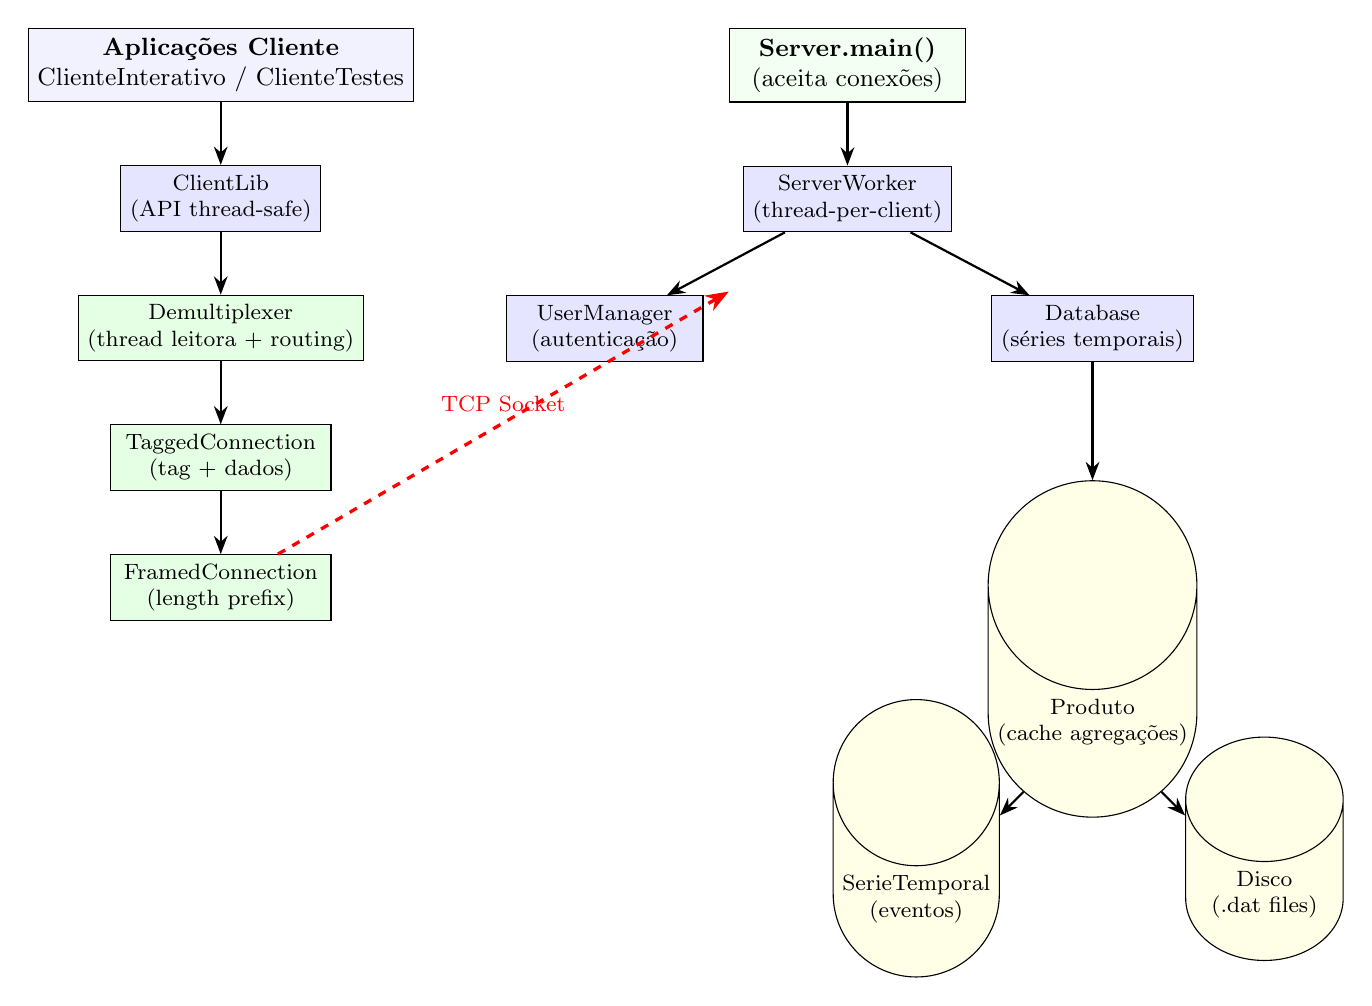
\begin{tikzpicture}[
    node distance=0.8cm,
    box/.style={rectangle, draw, minimum width=3cm, minimum height=0.8cm, align=center, font=\small},
    component/.style={rectangle, draw, minimum width=2.5cm, minimum height=0.7cm, align=center, font=\footnotesize, fill=blue!10},
    layer/.style={rectangle, draw, minimum width=2.8cm, minimum height=0.7cm, align=center, font=\footnotesize, fill=green!10},
    storage/.style={cylinder, draw, shape border rotate=90, minimum width=2cm, minimum height=0.6cm, align=center, font=\footnotesize, fill=yellow!10},
    arrow/.style={-Stealth, thick}
]

% CLIENTE
\node[box, fill=blue!5] (apps) {\textbf{Aplicações Cliente}\\ClienteInterativo / ClienteTestes};
\node[component, below=of apps] (clientlib) {ClientLib\\(API thread-safe)};
\node[layer, below=of clientlib] (demux) {Demultiplexer\\(thread leitora + routing)};
\node[layer, below=of demux] (tagged) {TaggedConnection\\(tag + dados)};
\node[layer, below=of tagged] (framed) {FramedConnection\\(length prefix)};

% SERVIDOR
\node[box, fill=green!5, right=4cm of apps] (server) {\textbf{Server.main()}\\(aceita conexões)};
\node[component, below=of server] (worker) {ServerWorker\\(thread-per-client)};
\node[component, below left=0.8cm and 0.5cm of worker] (usermgr) {UserManager\\(autenticação)};
\node[component, below right=0.8cm and 0.5cm of worker] (database) {Database\\(séries temporais)};
\node[storage, below=1.5cm of database] (produto) {Produto\\(cache agregações)};
\node[storage, below left=0.3cm and 0.3cm of produto] (serie) {SerieTemporal\\(eventos)};
\node[storage, below right=0.3cm and 0.3cm of produto] (disco) {Disco\\(.dat files)};

% Conexões Cliente
\draw[arrow] (apps) -- (clientlib);
\draw[arrow] (clientlib) -- (demux);
\draw[arrow] (demux) -- (tagged);
\draw[arrow] (tagged) -- (framed);

% Conexão TCP
\draw[arrow, dashed, red, very thick] (framed) -- node[above, font=\footnotesize] {TCP Socket} ($(server.south west) + (0,-2.4)$);

% Conexões Servidor
\draw[arrow] (server) -- (worker);
\draw[arrow] (worker) -- (usermgr);
\draw[arrow] (worker) -- (database);
\draw[arrow] (database) -- (produto);
\draw[arrow] (produto) -- (serie);
\draw[arrow] (produto) -- (disco);

\end{tikzpicture}
\caption{Arquitetura do Sistema Distribuído de Séries Temporais}
\label{fig:arquitetura}
\end{figure}

\subsection{Estratégia de Locking Hierárquico}

Para minimizar contenção, implementámos locking em 3 níveis:

\textbf{Nível 1 - Database}: Lock global para operações estruturais (por ex para novoDia). Mantido brevemente para obter referências e libertado depois antes de fazer cálculos.

\textbf{Nível 2 - SerieTemporal}: Cada dia tem o seu lock. Isto permite paralelismo entre operações em dias diferentes.

\textbf{Nível 3 - Produto}: Cada produto tem lock próprio para a cache. Cálculos pesados como (iterar eventos) ocorrem \textit{fora} do lock, apenas a verificação/armazenamento de cache usa esta sincronização.

Esta estratégia permite que múltiplas threads processem produtos ou dias diferentes sem interferência.

\subsection{Prevenção de Race Conditions}

O método \texttt{registarUser()} do \texttt{UserManager} previne TOCTOU (Time-Of-Check-Time-Of-Use) realizando verificação e inserção atomicamente dentro do mesmo bloco protegido:

\begin{lstlisting}[language=Java]
lock.lock();
try {
    if (utilizadores.containsKey(username)) 
        return false;
    utilizadores.put(username, new User(username, password));
    return true;
} finally {
    lock.unlock();
}
\end{lstlisting}

Sem esta atomicidade, existiria a possibilidade de duas threads verificarem simultaneamente que o utilizador não existe e ambas inseri-lo, causando sobrescrita.

\section{Agregações com Cache Lazy}

\subsection{Estratégia On-Demand}

As agregações (quantidade, volume, preço médio, máximo) são calculadas apenas quando solicitadas pela primeira vez para cada combinação produto-dias. O resultado é guardado em cache no objeto \texttt{Produto}, indexado por uma chave composta: \texttt{"operacao\_dias"} (ex: \texttt{"qtd\_7"}).

O padrão implementado tem 3 fases:
\begin{enumerate}[noitemsep]
    \item \textbf{Check cache} (com lock): Se existe, retorna imediatamente
    \item \textbf{Calculate} (SEM lock): Itera sobre séries temporais
    \item \textbf{Store} (com lock): Guarda resultado na cache
\end{enumerate}

\subsection{Invalidação de Cache}

A cache é invalidada no \texttt{novoDia()} através do método \texttt{invalidarCaches()} da \texttt{Database}, que percorre todos os produtos e limpa os seus HashMaps de cache. Esta estratégia é adequada pois:
\begin{itemize}[noitemsep]
    \item \texttt{novoDia()} é uma operação menos utilizada (comparada a consultas)
    \item Garantia de consistência: se executarmos uma nova consulta recalcula com dados já atualizados
\end{itemize}

\subsection{Performance}

Os testes que realizámos demonstraram um speedup de \textbf{10-50x} entre um cache hit (0.1-0.2ms) e uma cache miss (2-5ms), o que nos mostrou que valeu a pensa implementar esta estratégia.

\section{Serialização Eficiente (Fase 4)}

Para evitar enviar strings repetidas ao filtrar eventos, implementámos um protocolo com dicionário de produtos inspirado em técnicas de compressão:

\begin{enumerate}[noitemsep]
    \item Servidor identifica produtos únicos na lista de eventos
    \item Envia dicionário: \texttt{numProdutos + [produto UTF] * numProdutos}
    \item Envia eventos com índices: \texttt{numEventos + [índice, qtd, preço, timestamp] * numEventos}
\end{enumerate}

\textbf{Ganho}: Desta maneira, para 100 eventos de "Laptop" (7 bytes UTF), economizamos $100 \times 7 - 7 = 693$ bytes ( +/- 99\% de redução do tamanho na transmissão do nome).

\section{Barreiras com Conditions (Fase 5)}

\subsection{Vendas Simultâneas}

A \texttt{Database} mantém uma lista de pedidos pendentes (\texttt{PedidoVendasSimultaneas}). Cada \texttt{adicionarEvento()} verifica se satisfaz algum pedido. Usamos também o \texttt{Condition.await()} e \texttt{signalAll()} para acordar threads.

Antes de bloquear, verificamos se os dois produtos já foram vendidos hoje. Se sim, retornamos imediatamente sem await().

\subsection{Vendas Consecutivas}

Mantemos um contador por produto (\texttt{vendasConsecutivasPorProduto}). Ao adicionar um evento, incrementamos o contador do produto e zeramos os restantes. Quando o contador atinge n, \texttt{signalAll()} acorda todas as threads que estavam adormecidas.

\textbf{Trade-off}: Usamos \texttt{signalAll()} em vez de \texttt{signal()} para garantir corretude (todas as threads verificam condição), embora acorde threads desnecessariamente.

\section{Persistência com LRU (Fase 7)}

\subsection{Gestão de Memória}

Para esta fase, usamos o \texttt{LinkedHashMap} com \texttt{accessOrder=true} (true significa que segue LRU) para implementar a cache LRU automática. O método \texttt{removeEldestEntry()} é sobrescrito para dar trigger ao \texttt{saveToFile()} quando o tamanho excede S:

\begin{lstlisting}[language=Java]
memoriaCache = new LinkedHashMap<>(S, 0.75f, true) {
    protected boolean removeEldestEntry(Map.Entry e) {
        if (size() > S) {
            SerieTemporal serie = (SerieTemporal) e.getValue();
            serie.saveToFile(PATHDADOS + "dia_" + 
                serie.getDia() + ".dat");
            return true;
        }
        return false;
    }
};
\end{lstlisting}

\subsection{Estratégia Híbrida}

Quando uma agregação necessita de mais do que S dias:
\begin{enumerate}[noitemsep]
    \item Carrega até S séries em cache (LRU normal)
    \item Deteta o limite atingido (\texttt{memoriaCache.size() >= S})
    \item De seguida, processa os dias restantes em streaming. Ou seja, lê evento-a-evento do disco, agrega, e de seguida descarta (sem carregar para a memória)
\end{enumerate}

Esta abordagem permitiu agregar sobre \textbf{todos os D dias} usando apenas \textbf{S séries simultâneas} em memória.

\section{Avaliação de Desempenho}

\subsection{Metodologia}

Para esta fase, implementamos inúmeros testes a várias funcionalidades do nosso sistema em \texttt{ClienteTestes.java} dividida em 4 categorias: funcionais, performance, escalabilidade e robustez. Para a realização destes testes, iniciamos o servidor com D=50, S=10. O hardware utilizado para fazer estes testes foi o seguinte: cpu Intel i7-1360P, 16GB RAM, Linux, JVM OpenJDK 21.

\subsection{Resultados}

\textbf{Performance}:
\begin{itemize}[noitemsep]
    \item Inserção: 35.000 eventos/s
    \item Persistência: 28ms/dia médio
    \item Cache hit: 10-50x mais rápido que cache miss (já mencionado antes)
\end{itemize}

\textbf{Escalabilidade Multi-Cliente}:
\begin{center}
\begin{tabular}{|c|c|c|}
\hline
Clientes & Throughput (ops/s) & Speedup \\
\hline
1 & 7.692 & 1.0x \\
5 & 35.714 & 4.6x \\
10 & 71.428 & 9.3x \\
20 & 60.606 & 7.9x \\
\hline
\end{tabular}
\end{center}

O speedup de \textbf{9.3x com 10 clientes} demonstrou uma escalabilidade quase linear. Depois com 20 clientes degradou um pouco, o que indicou uma contenção na Database começando a afetar a performance.
Além disso, devido à arquitetura utilizada thread-per-connection, seria esperado um resultado semelhante já que embora seja de fácil implementação, apresenta alguns problemas de escabilidade devido à limitação do hardware.

\textbf{Multi-Threaded (1 cliente, 10 threads)}: 7.843 ops/s. Inferior a 10 clientes separados devido a gargalo na socket partilhada, mas valida funcionamento correto do Demultiplexer.

\textbf{Robustez}:
Testamos um cliente normal e outro cliente lento iniciado primeiro mas com sleeps para ver se atrasava o outro. Testamos também desconectar um cliente a meio de operações para ver se gerava problemas ou crashava o servidor.
\begin{itemize}[noitemsep]
    \item O cliente lento (500ms/op) não bloqueou o cliente normal (36ms total para 100 ops)
    \item O servidor sobreviveu a desconexões abruptas sem crash
\end{itemize}

\section{Conclusões}

O sistema implementa com sucesso todas as 7 fases solicitadas, demonstrando:

\begin{itemize}[noitemsep]
    \item \textbf{Corretude}: Os testes funcionais validaram a autenticação, agregações, barreiras, filtros, e persistência
    \item \textbf{Escalabilidade}: Existiu um speedup de +/- 9.3x até 10 clientes concorrentes
    \item \textbf{Eficiência}: A cache é 10-50x mais rápida, com uma serialização eficiente, e streaming para grandes datasets
    \item \textbf{Robustez}: implementamos isolamento entre clientes, e recuperação de desconexões
\end{itemize}

De forma geral, o nosso grupo desenvolveu um bom trabalho que responde aos requisitos necessários pedidos no enunciado. As decisões de design que tomámos, como o locking hierárquico em 3 níveis e a cache lazy on-demand, mostraram-se eficazes através dos testes quantitativos realizados. O sistema está preparado para cenários de produção onde D $\gg$ S, mantendo a performance previsível através de gestão inteligente de memória com LRU e paralelismo efetivo. Finalmente, a arquitetura de 3 camadas para clientes multi-threaded, embora tenha adicionado complexidade, permitiu cumprir os requisitos da Fase 6 mantendo a corretude do sistema mesmo sob carga concorrente elevada.

\end{document}